\documentclass{article}

%
% 引入模板的style文件
%
\usepackage{homework}

\setCJKmainfont{SimSun}[AutoFakeBold] %宋体加粗
\setCJKsansfont{SimHei}[AutoFakeBold] %黑体加粗


\usepackage{minted} %配合minted宏包进行好看的高亮
\usepackage{currfile} %配合minted宏包进行好看的高亮
\usepackage{caption} %配合minted宏包进行好看的高亮
\usepackage{tcolorbox} %配合minted宏包进行好看的高亮
\usepackage{xcolor} %配合minted宏包进行好看的高亮
\tcbuselibrary{skins} %配合minted宏包进行好看的高亮
\tcbuselibrary{minted} %配合minted宏包进行好看的高亮
\usemintedstyle{paraiso-dark} %配合minted宏包进行好看的高亮



%
% 封面
%

\title{
	
\includegraphics[width=0.6\textwidth]{images/title/ucas_logo 1.pdf}\\
    \vspace{1in}
    \textmd{\textbf{\hmwkClass}}\\
	\textmd{\Large{\textbf{\hmwkClassID}}}\\
    \textmd{\textbf{\hmwkTitle}}\\
    \normalsize\vspace{0.1in}\large{\hmwkCompleteTime }\\
    \vspace{0.1in}\large{\textit{\hmwkClassInstructor\ }}\\
    \vspace{1in}
	
\includegraphics[width=0.25\textwidth]{images/title/Cyber.jpg}\\
	\vspace{1in}
}


\author{
	\hmwkAuthorName \\ 
	\hmwkAuthorStuID \\
	\hmwkAuthorInst \\
	\hmwkAuthorzhuanye \\
	\hmwkAuthorfangxiang
	}
\date{}

\renewcommand{\part}[1]{\textbf{\large Part \Alph{partCounter}}\stepcounter{partCounter}\\}


%
% 正文部分
%
\begin{document}


\maketitle


%\include{chapters/ch01}
%\include{chapters/ch02}
%\include{chapters/ch03}
%\include{chapters/ch04}
%\include{chapters/ch05}


\begin{homeworkProblem}
	自己编程实现课堂上Polynomial Curve Fitting的例子, 体会过拟合.
	\\

	\solution 先根据均匀分布$U(0,1)$随机产生10个数据点, 再利用函数$y(x)=\sin (2\pi x)$并添加高斯噪声(噪声均值为0, 方差为$\sigma^2=0.08^2$)产生对应的$y$数据. 我们分别用$M=0, 2 ,5 ,9$次多项式对上述产生的数据点进行多项式拟合. 具体的Matlab代码如下所示:
\begin{tcblisting}{listing engine=minted,boxrule=0.1mm,
colback=blue!5!white,colframe=blue!75!black,
listing only,left=5mm,enhanced,sharp corners=all,
overlay={\begin{tcbclipinterior}\fill[red!20!blue!20!white] (frame.south west)
rectangle ([xshift=5mm]frame.north west);\end{tcbclipinterior}},
minted language=matlab,
minted style=tango,
minted options={fontsize=\normalsize,breaklines,autogobble,linenos,numbersep=3mm}}
N = 10; %产生的数据点的个数
x = rand(10,1); %产生均匀分布U(0,1)的10个点
noise_sigma = 0.08; %噪声的方差为noise_sigma^2
M = 9;
y = sin(2*pi*x) + randn(10,1)*noise_sigma; %randn产生N(0,1)正态分布的数据
figure (1)
axis([0 1 -2 2])
plot(x, y, 'b.')
x_r = 0: 0.01: 1;
y_r = sin(2*pi*x_r);
hold on
plot(x_r, y_r, 'b'); %数据的真实曲线(蓝色的)
p_x = [];

for m = 0 : M
    p_x = [p_x, x.^m]; %产生[x^0;x^1;x^2,...,x^M]
end
p_x = p_x';
w = pinv(p_x*p_x')*p_x*y;
y_est = w'*p_x;
figure(1);
hold on
x_cur = 0:0.01:1;

y_cur = zeros(size(x_cur));
for m = 0 : M
    y_cur = y_cur + w(m + 1)*(x_cur.^m);
end
axis([0 1 -2 2])
plot(x_cur, y_cur, 'r') % 画出红色的拟合曲线
\end{tcblisting}
	代码的运行结果和具体的多项式曲线拟合情况见后页图\ref{M=0},\ref{M=2},\ref{M=3},\ref{M=4},\ref{M=5},\ref{M=9}中所示. 可以看出的是: 当$M=3,4,5$时, 过拟合效应较小, 当$M=9$(过大)时, 多项式拟合出现了强烈的过拟合现象.
	\newpage
	\begin{figure}[htbp]
		\centering
		\begin{minipage}{0.49\linewidth}
			\centering
			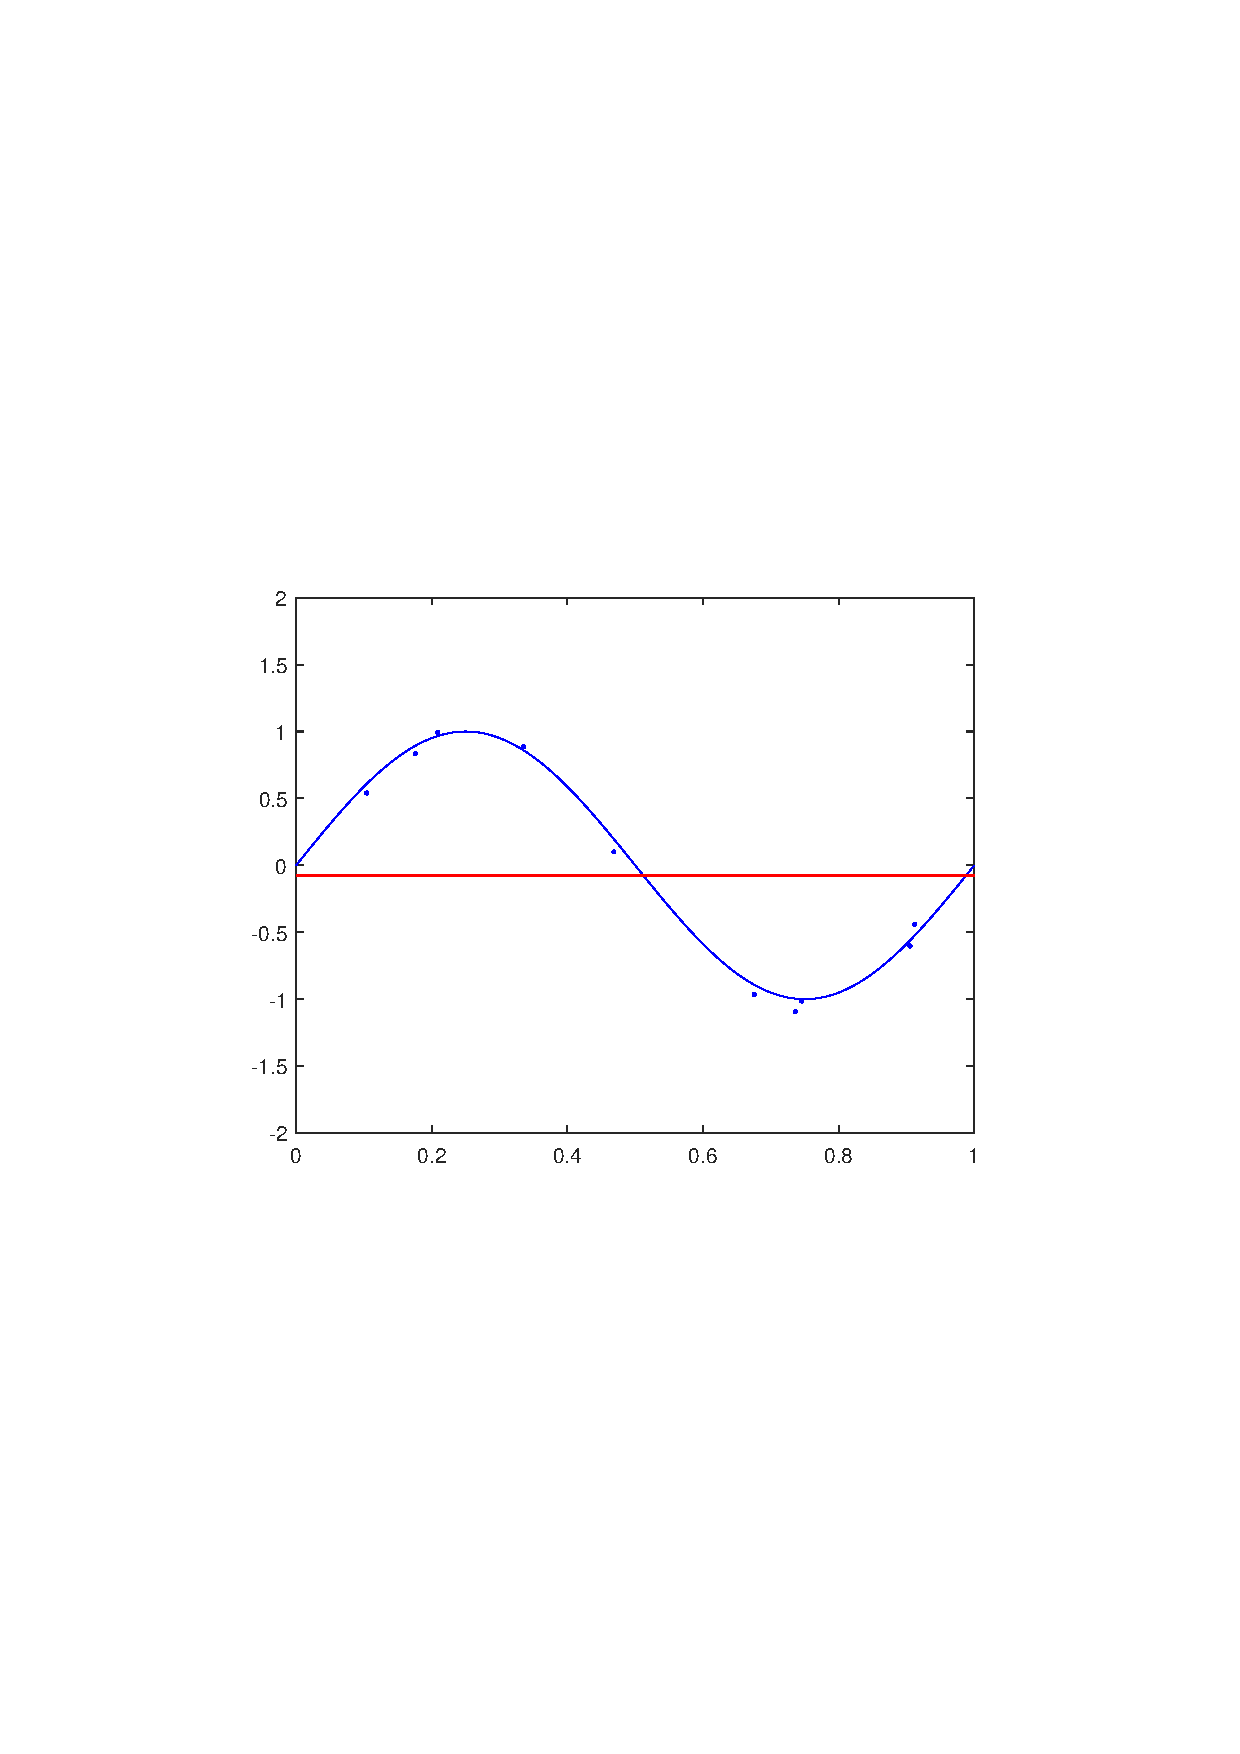
\includegraphics[width=0.9\linewidth]{images/title/M=0.pdf}
			\caption{$M=0$时的拟合情况}
			\label{M=0}%文中引用该图片代号
		\end{minipage}
		\begin{minipage}{0.49\linewidth}
			\centering
			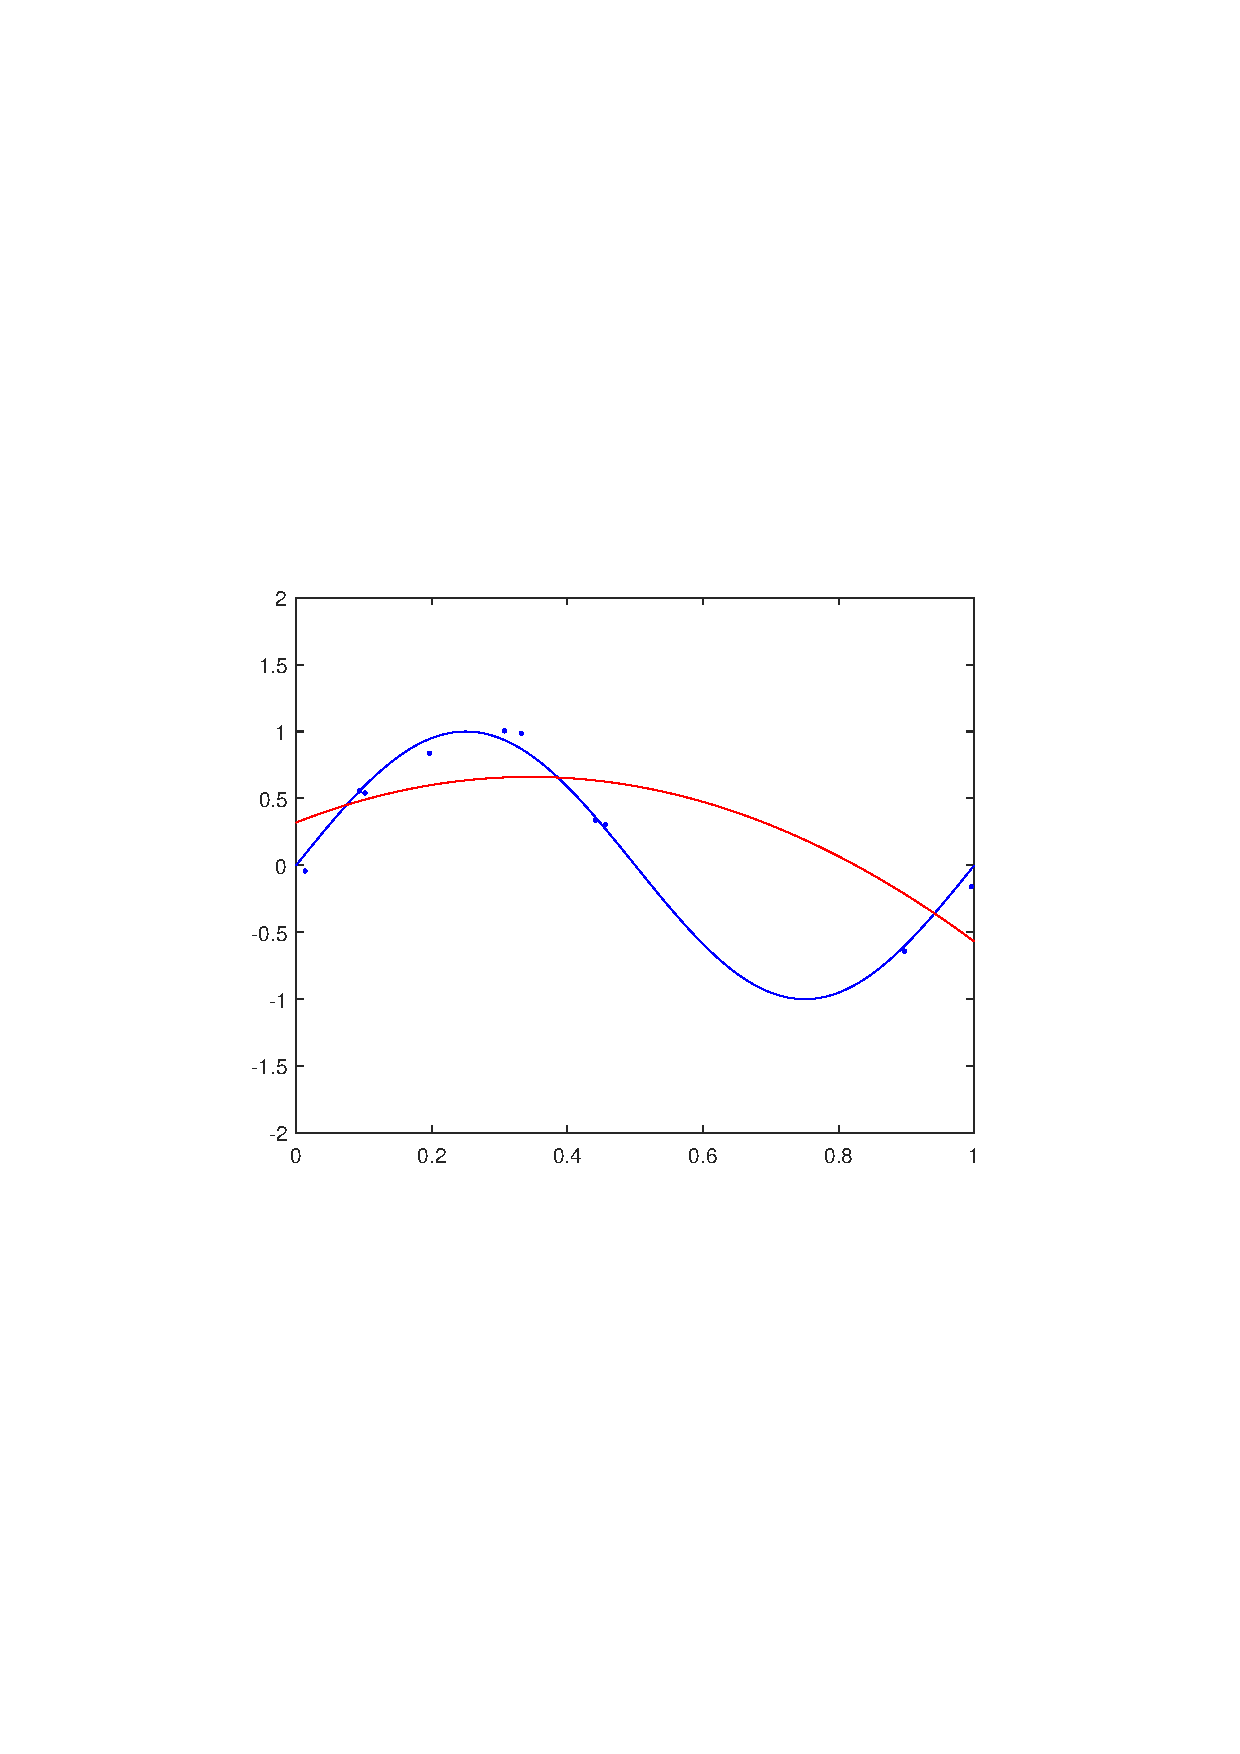
\includegraphics[width=0.9\linewidth]{images/title/M=2.pdf}
			\caption{$M=2$时的拟合情况}
			\label{M=2}%文中引用该图片代号
		\end{minipage}
		%\qquad
		%让图片换行,

		\begin{minipage}{0.49\linewidth}
			\centering
			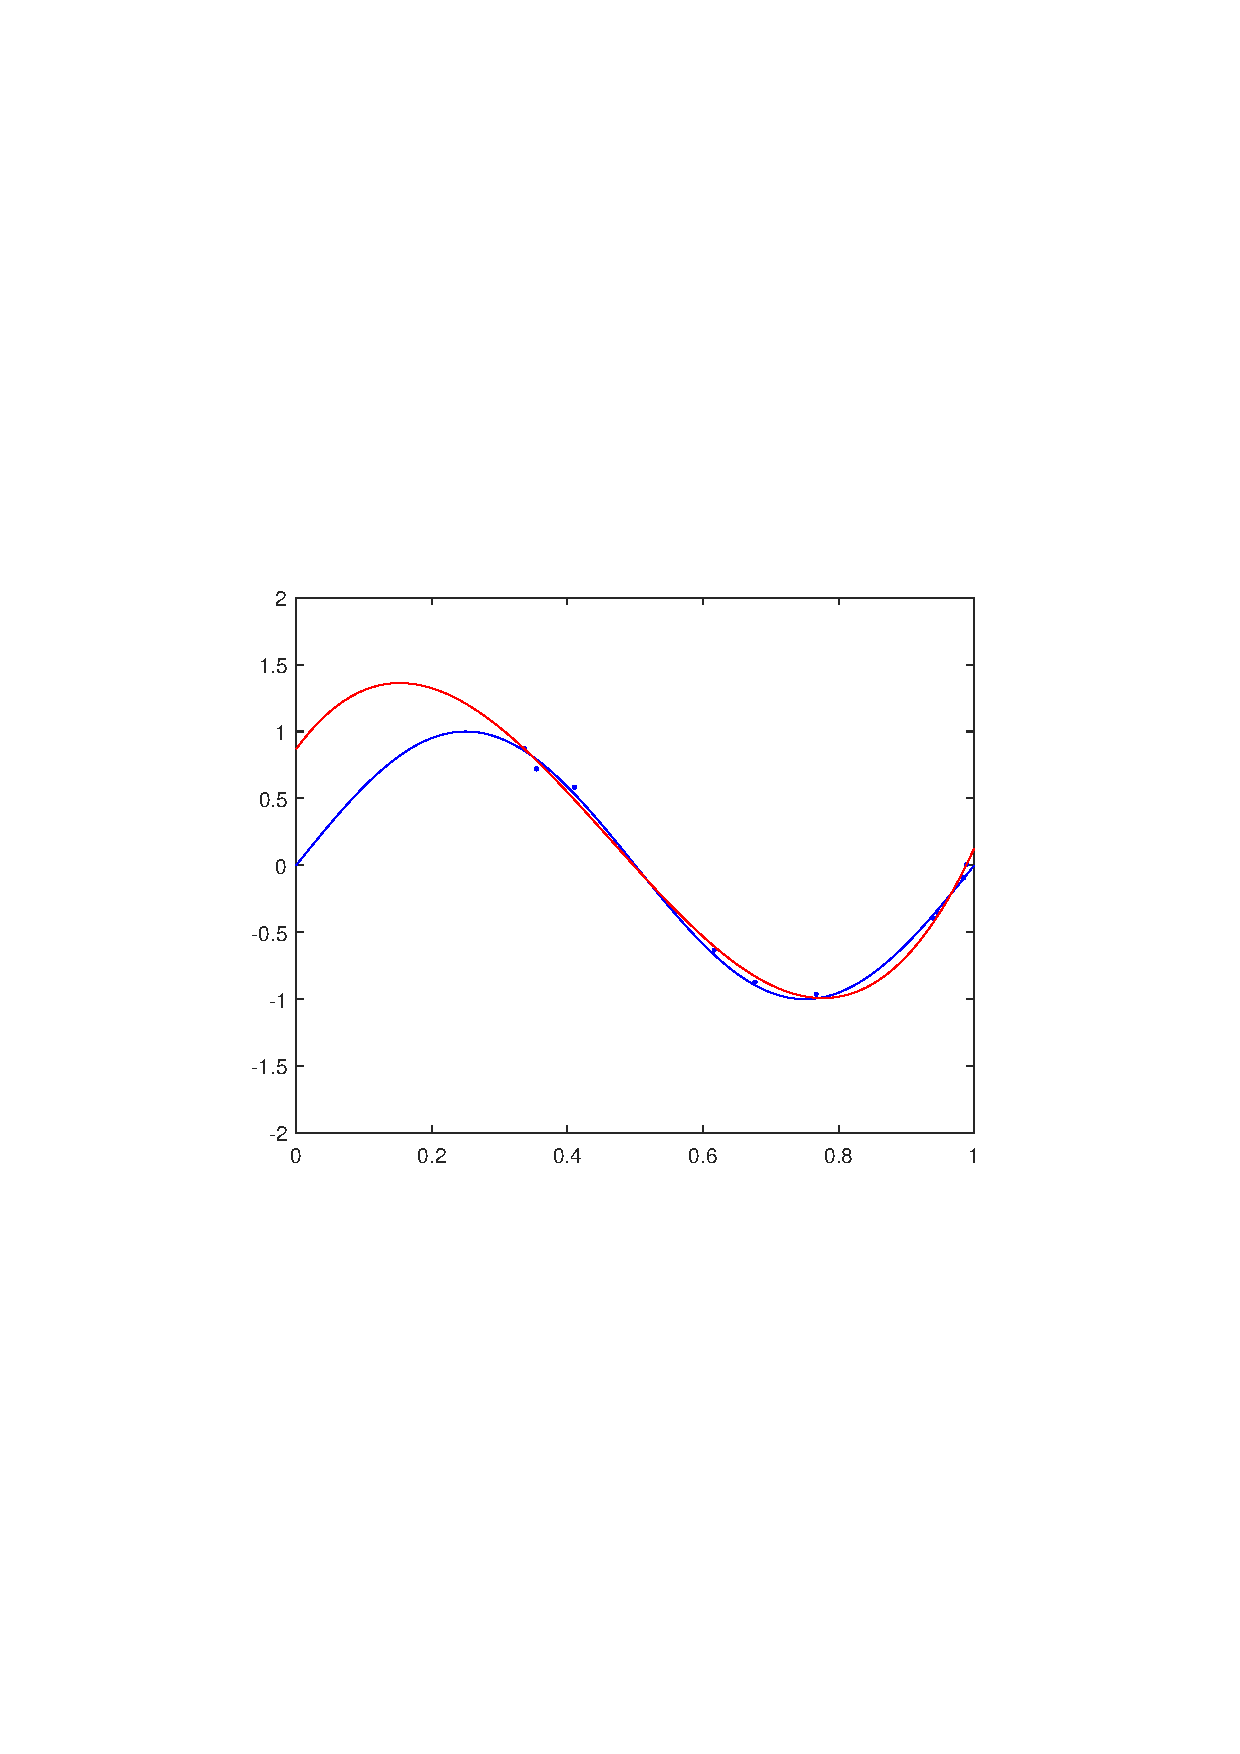
\includegraphics[width=0.9\linewidth]{images/title/M=3.pdf}
			\caption{$M=3$时的拟合情况}
			\label{M=3}%文中引用该图片代号
		\end{minipage}
		\begin{minipage}{0.49\linewidth}
			\centering
			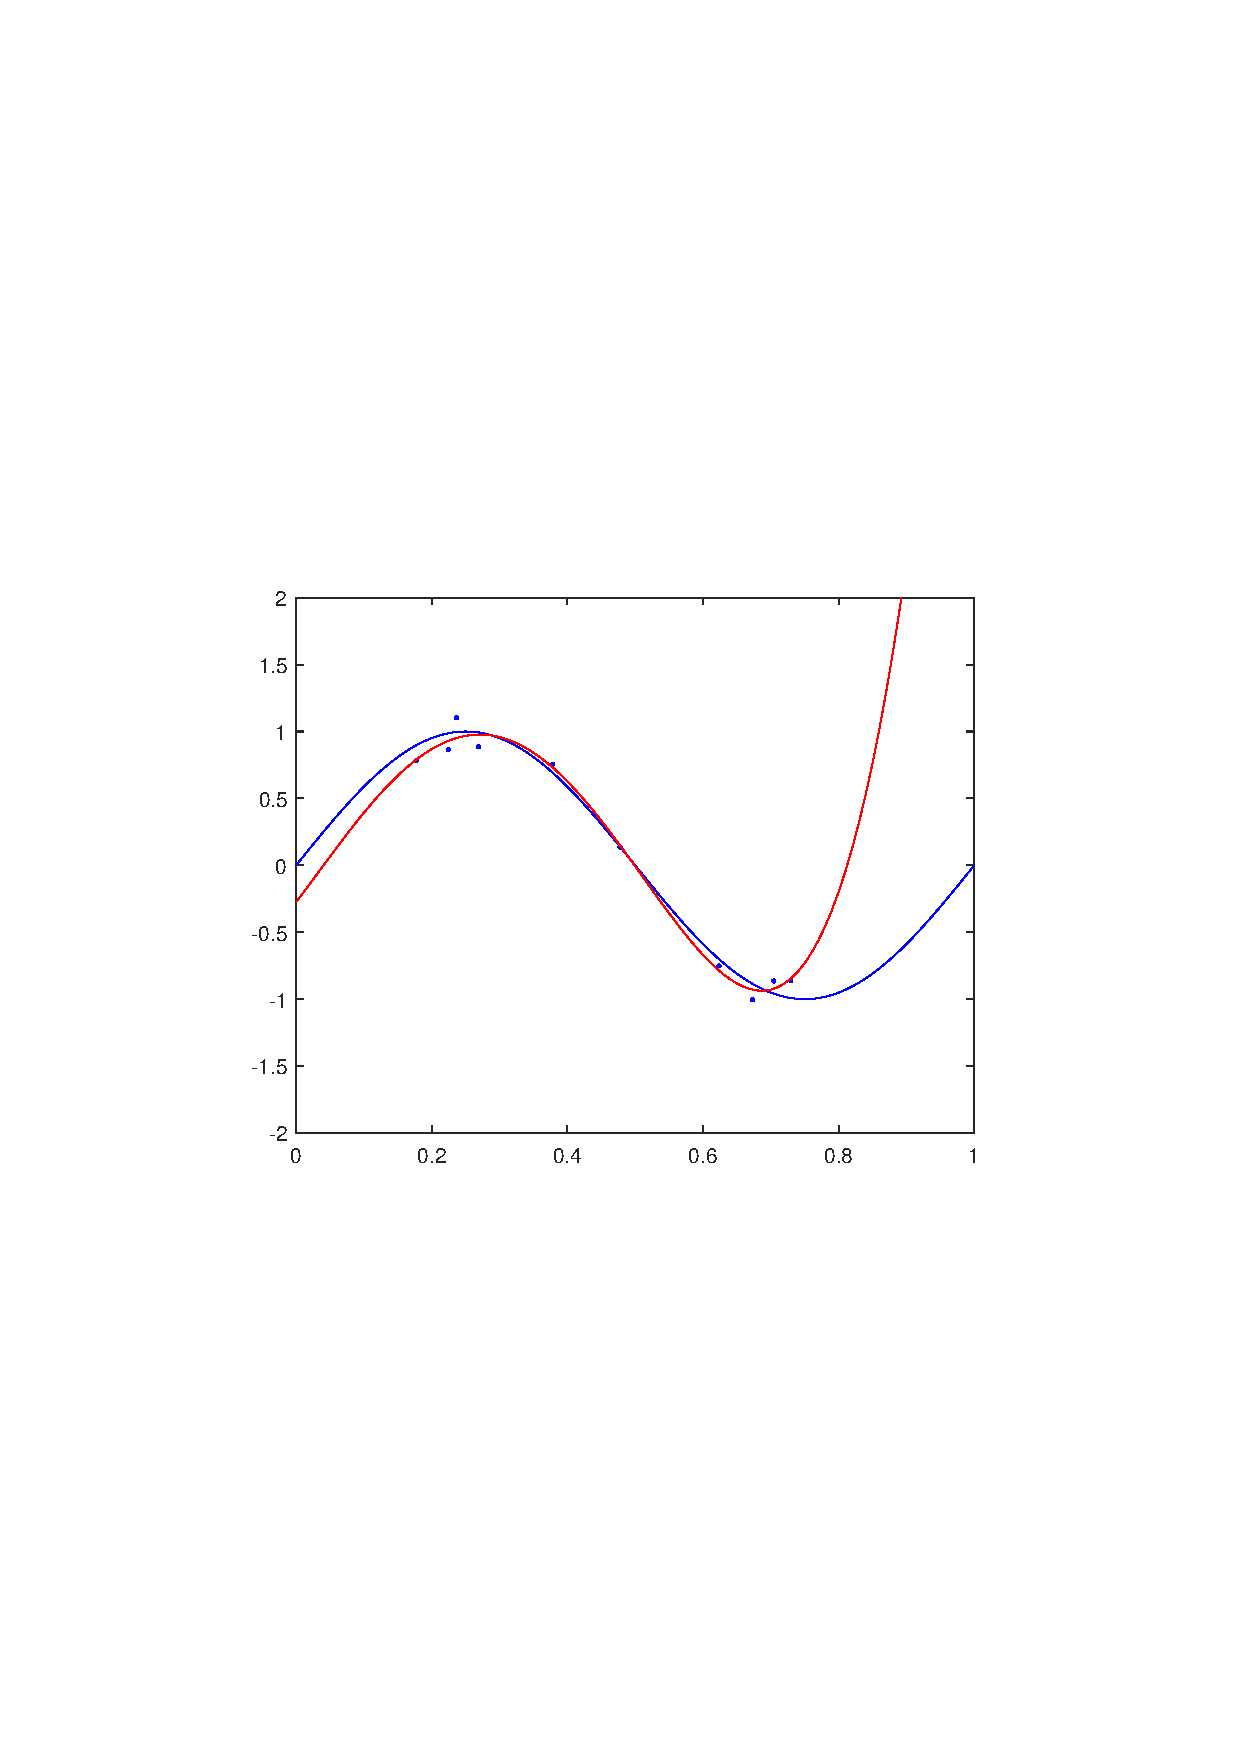
\includegraphics[width=0.9\linewidth]{images/title/M=4.pdf}
			\caption{$M=4$时的拟合情况}
			\label{M=4}%文中引用该图片代号
		\end{minipage}

		%\qquad
		%让图片换行,
		
		\begin{minipage}{0.49\linewidth}
			\centering
			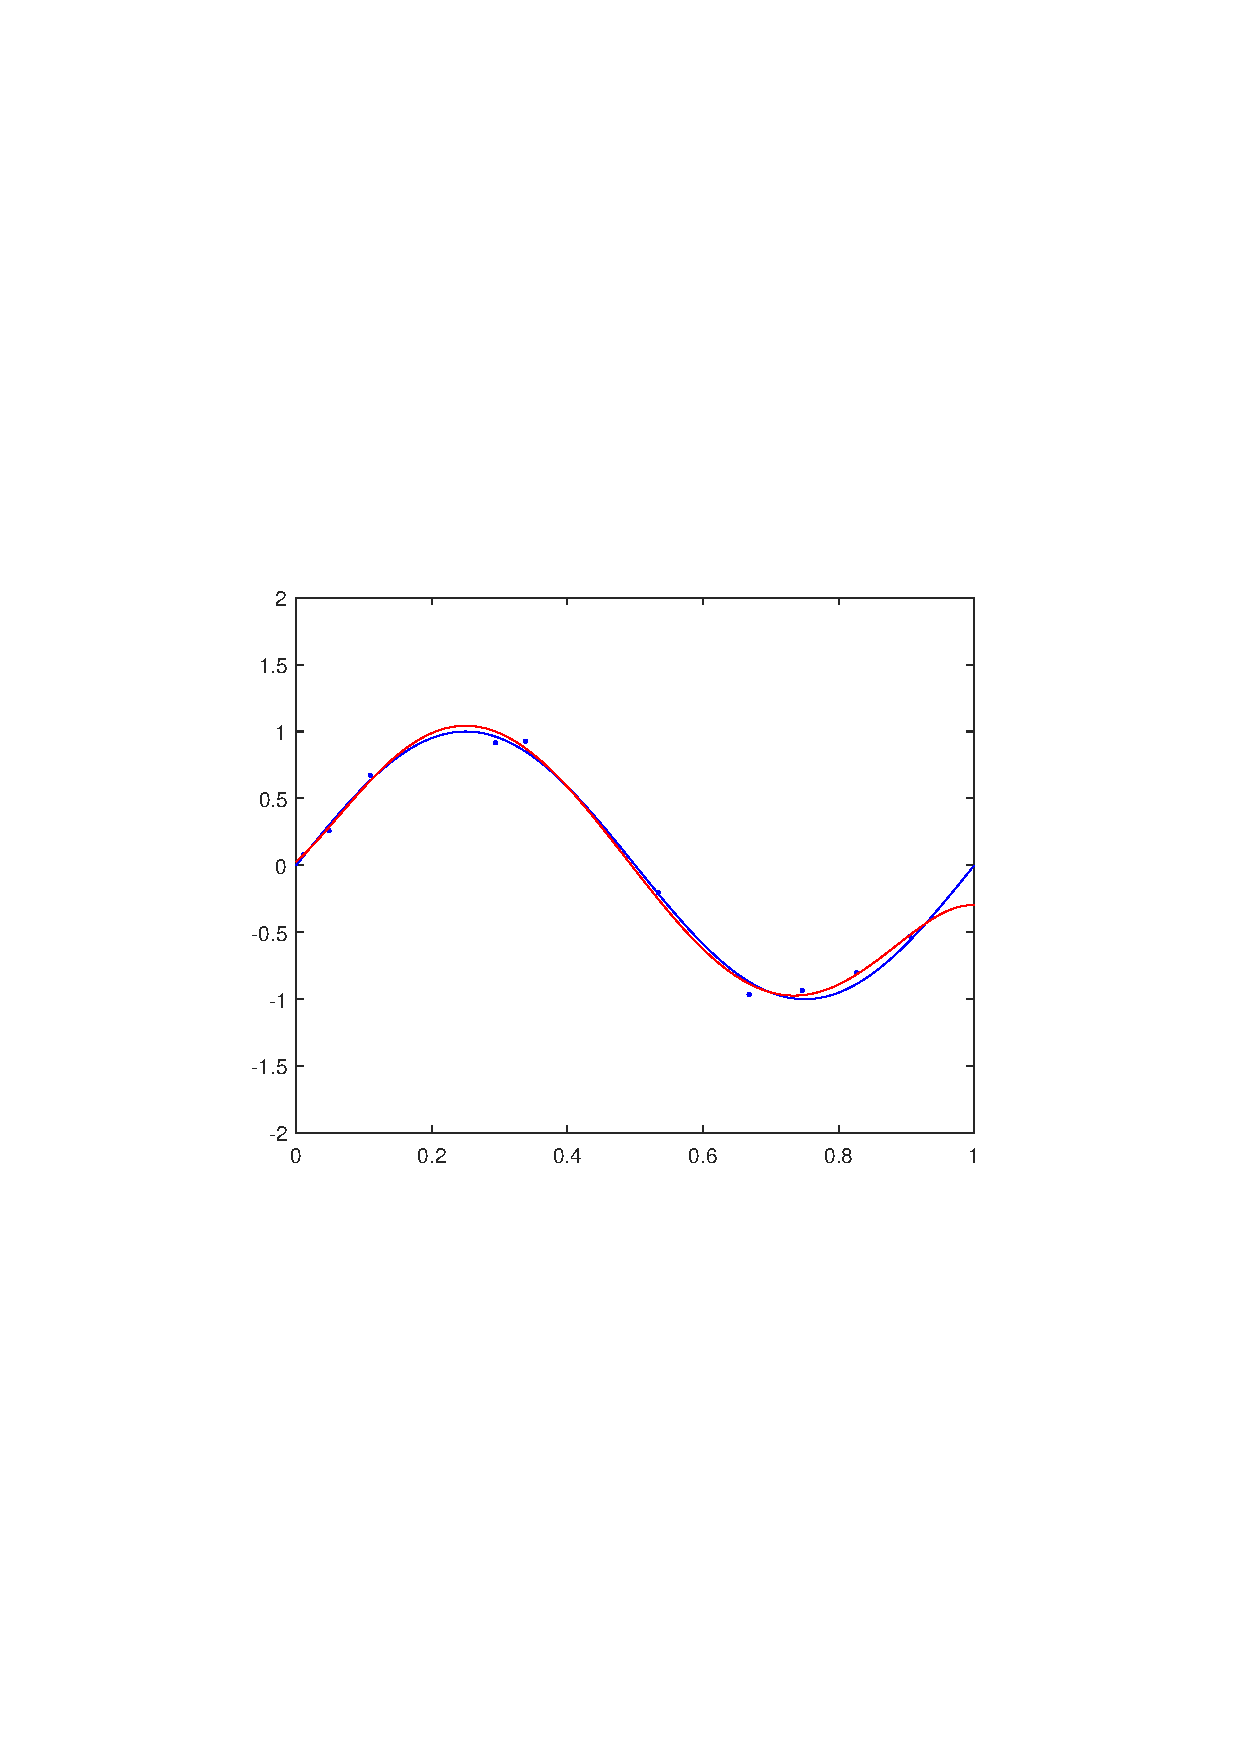
\includegraphics[width=0.9\linewidth]{images/title/M=5.pdf}
			\caption{$M=5$时的拟合情况}
			\label{M=5}%文中引用该图片代号
		\end{minipage}
		\begin{minipage}{0.49\linewidth}
			\centering
			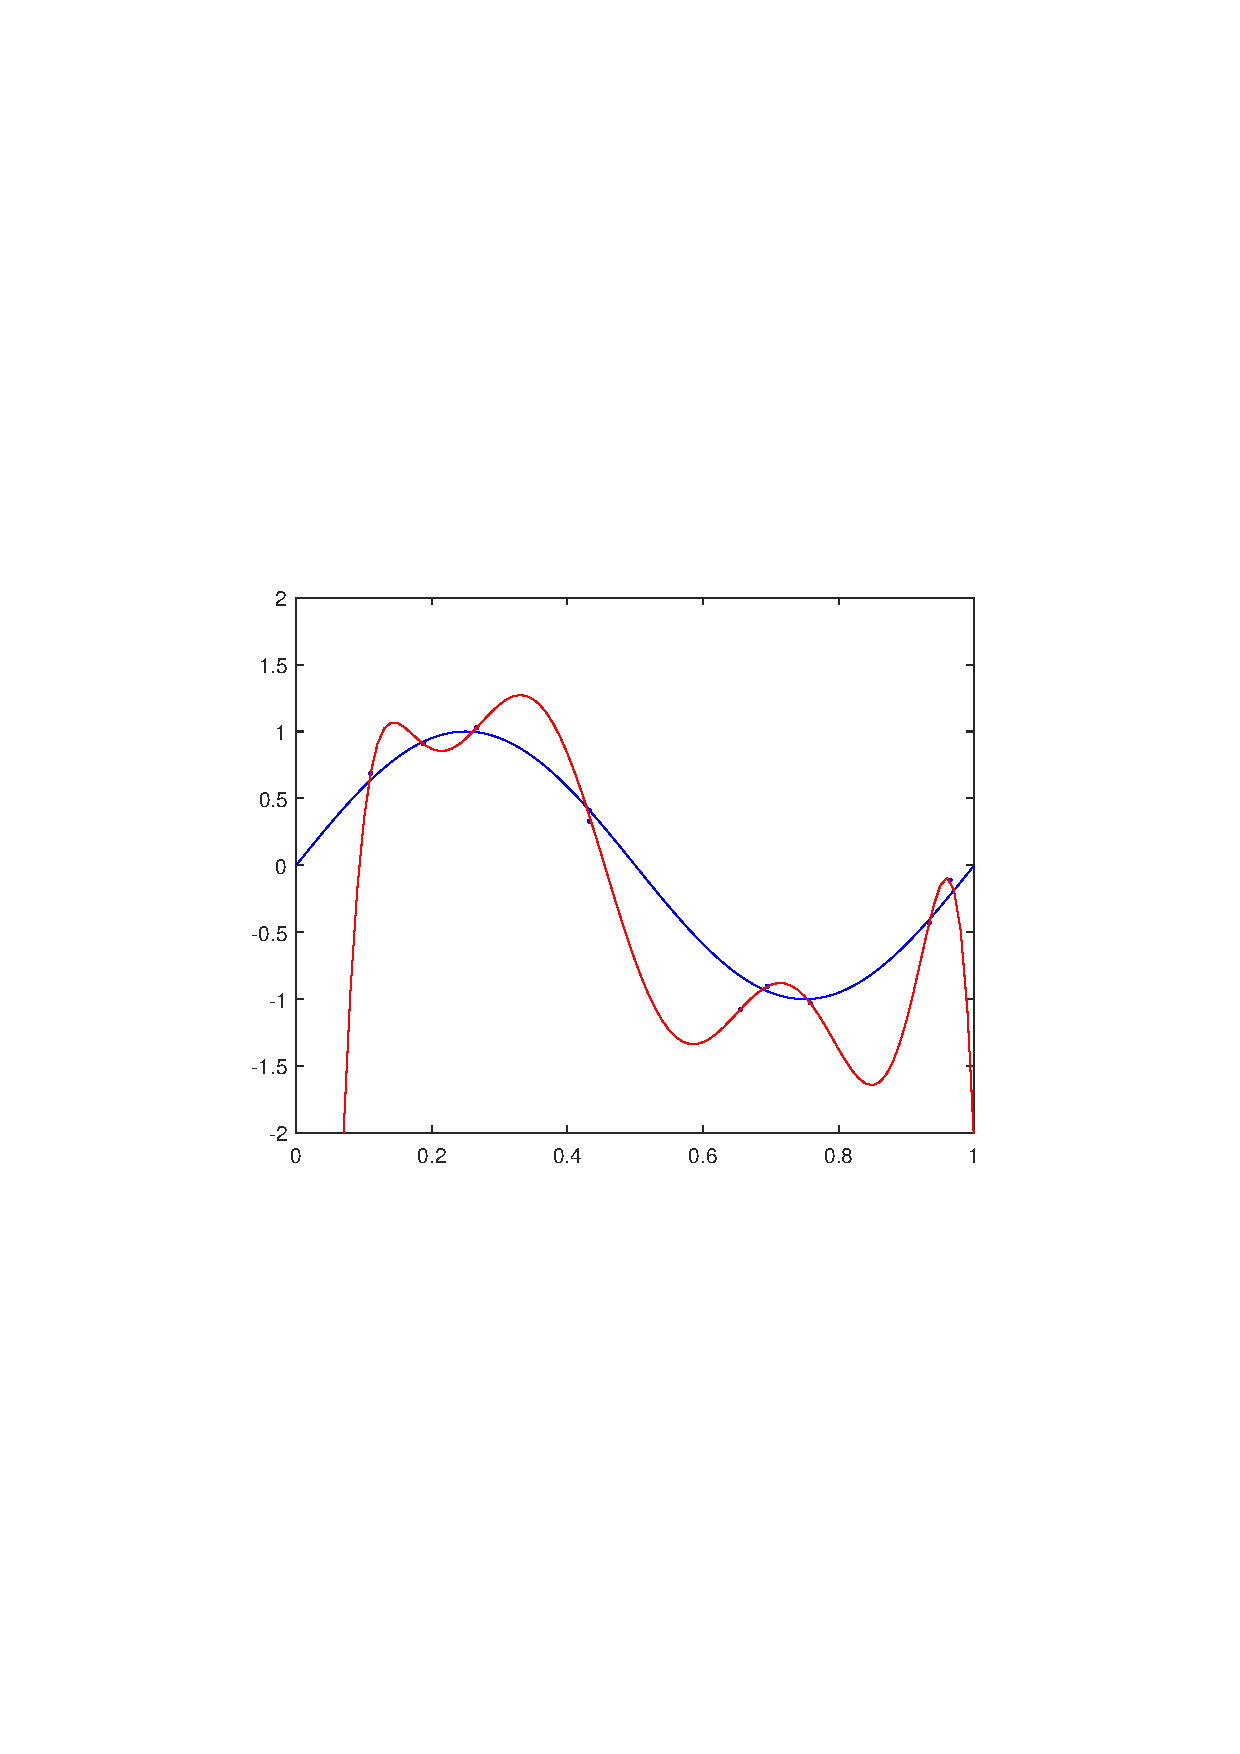
\includegraphics[width=0.9\linewidth]{images/title/M=9.pdf}
			\caption{$M=9$时的拟合情况}
			\label{M=9}%文中引用该图片代号
		\end{minipage}
	\end{figure}	
\end{homeworkProblem}


% 引用文献
%\bibliographystyle{unsrt}  % unsrt:根据引用顺序编号
%\bibliography{refs}


\end{document}
